\chapter{Versuch 5: Statistik}

\section{Einleitung}
Ziel dieses Versuches ist es die Wiederstände von 25 Wiederständen zu messen und
die vom Hersteller angegebene Toleranz zu überprüfen. Des Weiteren werden in diesem
Versuch statistische Momente berechnet, sowie die Siginifkanz dieser Abweichung am
Beispiel der beiden Grundschaltungen des Operationsverstärkers untersucht.

\section{Versuchsdurchführung}

\begin{tabular}[h]{c|c}
	Messung & Wiederstand in k$\Omega$ \\
	\hline
	1 & 3,895\\
	\hline
	2& 3,884\\
	\hline
	3 & 3,912\\
	\hline
	4 & 3,874\\
	\hline
	5& 3,881\\
	\hline
	6 & 3,878\\
	\hline
	7 & 3,889\\
	\hline
	8& 3,870\\
	\hline
	9 & 3,902\\
	\hline
	10 & 3,866\\
	\hline
	11& 3,997\\
	\hline
	12& 3,901
    \label{tab:Messreihe Wiederstände 1}
\end{tabular}
\begin{tabular}[h]{c|c}  
	13& 3,865\\
	\hline
	14& 3,920\\
	\hline
	15& 3,961\\
	\hline
	16& 3,870\\
	\hline
	17& 3,886\\
	\hline
	18& 3,878\\
	\hline
	19& 3,885\\
	\hline
	20& 3,901\\
	\hline
	21& 3,879\\
	\hline
	22& 3,957\\
	\hline
	23& 3,909\\
	\hline
	24& 3,935\\
	\hline
	25& 3,877
	\label{tab:Messreihe Wiederstände 2}
\end{tabular}

Angegeben wurden die Wiederstände von 3,9k$\Omega$ mit einer Genauigkeit von 5\%. 
Die Messung wurde mit einem Digital-Multimeter durchgeführt.

\subsection{Verteilung der Messwerte}

\begin{figure}[H]
	\centering
	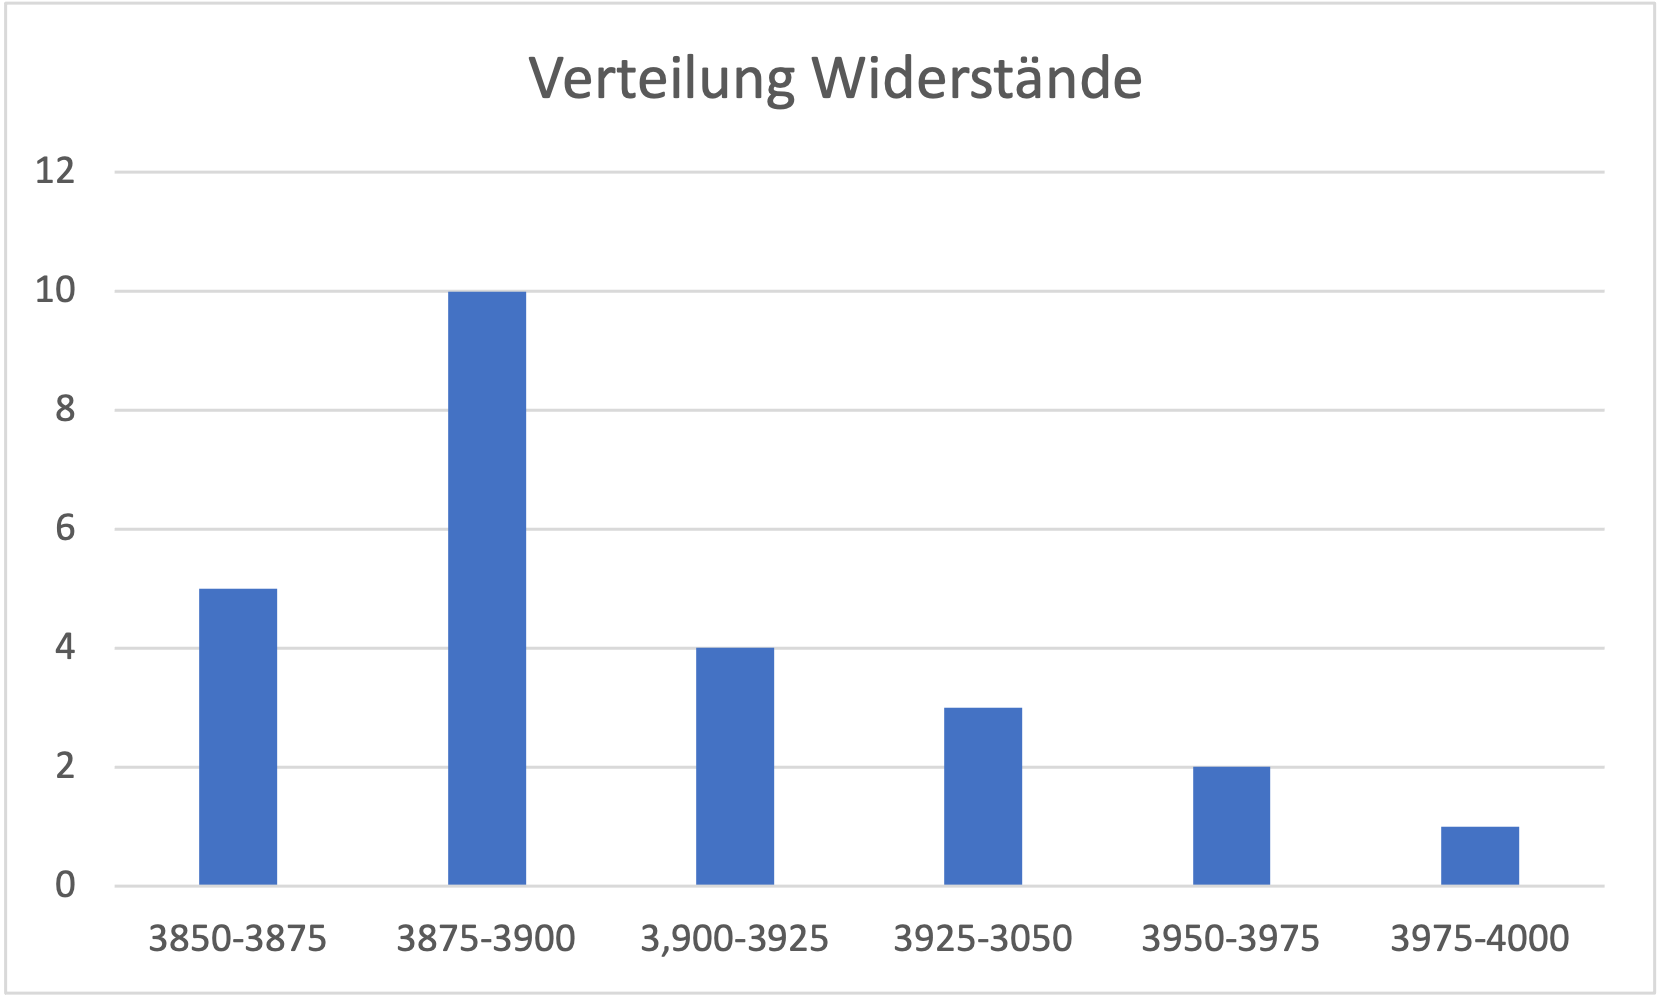
\includegraphics[height=7cm]{images/Versuch5/Verteilung_Widerstaende.png} 
	\caption{Verteilung der Wiederstände}
	\label{fig: Verteilung der Wiederstände}
\end{figure}

\section{Statistische Auswertung}

Den Mittelwert $\bar{R}$ berechnen wir mit folgender Formel:

\begin{equation}
	\bar{R} = \frac{1}{n} \sum_{i=1}^{n} R\textsubscript{i}
	\label{eq:R}
\end{equation}

Mit \ref*{eq:R} erhalten wir einen Mittelwert von $\bar{R}$ = 3,899k$\Omega$.

Die Standartavweichung $\sigma$ berechnet sich nach folgender Formel:

\begin{equation}
	\sigma = \sqrt{\frac{1}{n-1} \sum_{i=1}^{n} (R\textsubscript{i} - \bar{R})^2}
	\label{eq:Sigma}
\end{equation}

Durch einsetzen der Werte erhält man eine Standartavweichung von $\sigma$ = 0,03784k$\Omega$ 
= 37,84$\Omega$.
\subsection{Empirische Standartavweichung}

Die Abweichung entspricht somit 0,97\%. Die Herstellertoleranz ist somit 5,15
mal größer als die empirische Standartavweichung. Die Herstellertoleranz 
von 5\% ist groß angegeben, damit der Hersteller durch seine Angaben
kein Risiko eingeht, da durch Termperaturveränderungen größere Abweichungen
entstehen können.

\section{Operationsverstärker}

\subsection{Invertierender Verstärker}
\begin{figure}[H]
	\centering
	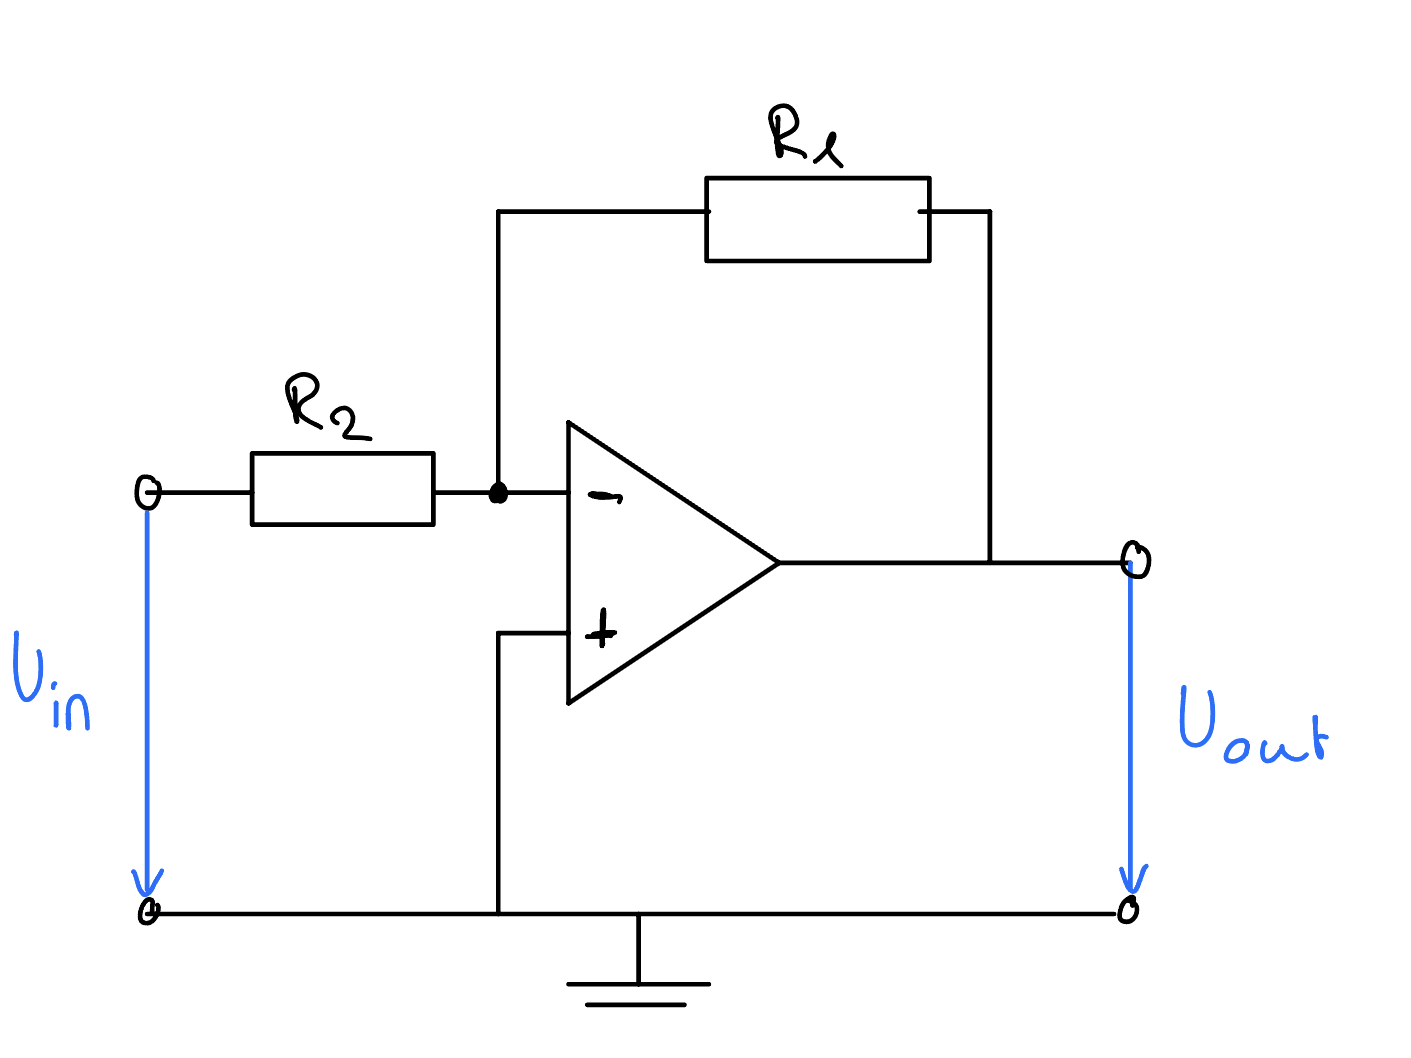
\includegraphics[height=7cm]{images/Versuch5/invertierend-opamp.jpeg} 
	\caption{Invertierender Operationsverstärker}
	\label{fig: Invertierender Operationsverstärker}
\end{figure}
Die Spannungverstärkung A\textsubscript{V} berechnet sich nach folgender Formel:
\begin{equation}
	A\textsubscript{V} = - \frac{R\textsubscript{1}}{R\textsubscript{2}}
	\label{eq:AV2}
\end{equation}
Durch das Verwenden des Wiederstands R\textsubscript{1}' = R\textsubscript{1} +- $\Delta$R 
ergibt sich folgende Formel für $\Delta$A\textsubscript{V}':
\begin{equation}
	\Delta A\textsubscript{V}' = - \frac{\Delta R}{R\textsubscript{1}}
	\label{eq:AV2'}
\end{equation}
Hier bleibt die relative Verstärkerungsänderung konstant:
\begin{equation}
	\frac{\Delta A\textsubscript{V}'}{A\textsubscript{V}'} = \frac{\Delta R}{R\textsubscript{1}} = \frac{0,05 * R\textsubscript{1}}{R\textsubscript{1}} = 5\%
	\label{eq:AV2''}
\end{equation}

\subsection{Nicht-Invertierender Verstärker}
\begin{figure}[H]
	\centering
	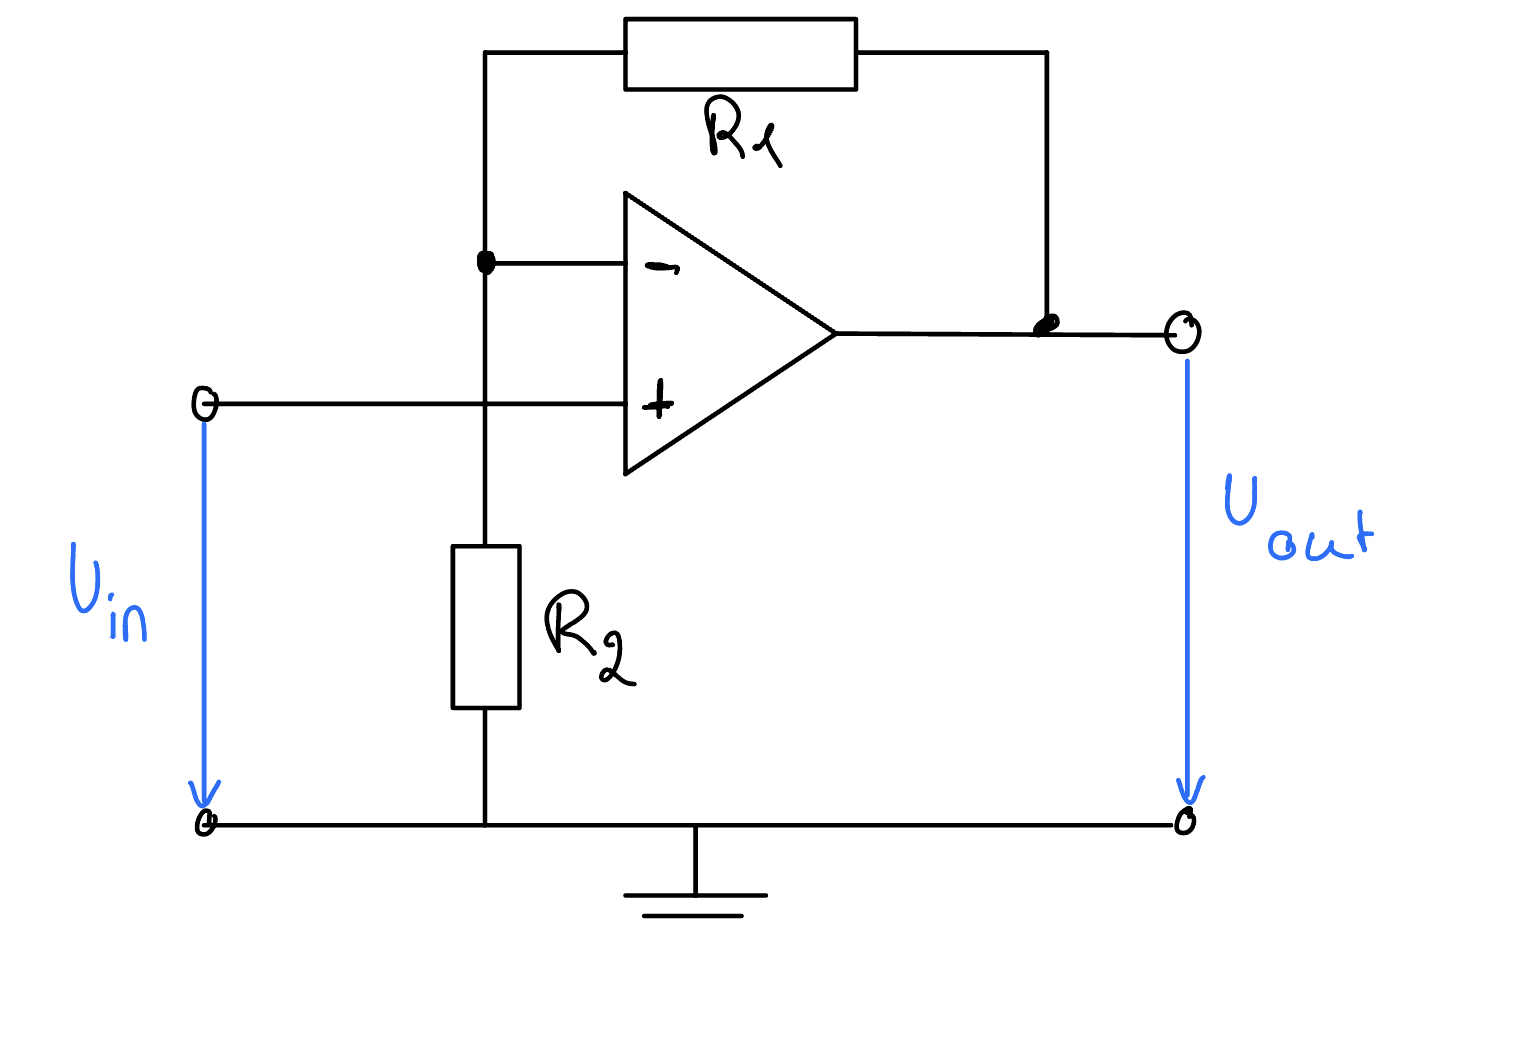
\includegraphics[height=7cm]{images/Versuch5/nicht-invertierend-opamp.jpeg} 
	\caption{Nicht-Invertierender Operationsverstärker}
	\label{fig: Nicht-Invertierender Operationsverstärker}
\end{figure}
Die Spannungverstärkung A\textsubscript{V} berechnet sich nach folgender Formel:
\begin{equation}
	A\textsubscript{V} = 1 + \frac{R\textsubscript{1}}{R\textsubscript{2}}
	\label{eq:AV}
\end{equation}
Durch das Verwenden des Wiederstands R\textsubscript{1}' = R\textsubscript{1} +- $\Delta$R 
ergibt sich folgende Formel für $\Delta$A\textsubscript{V}:
\begin{equation}
	\Delta A\textsubscript{V} = 1 + \frac{\Delta R}{R\textsubscript{1}+ R\textsubscript{2}}
	\label{eq:AV'}
\end{equation}

Mit Anwendung der Formel \ref*{eq:AV'} können wir die relative Verstärkerungsänderung
berechnen (R\textsubscript{1} = 1k$\Omega$,R\textsubscript{2} = 1k$\Omega$):

\begin{equation}
	\frac{\Delta A\textsubscript{V}}{A\textsubscript{V}}
	= \frac{\Delta R\textsubscript{1}}{R\textsubscript{1} + R\textsubscript{2}}
	= \frac{5\% * 1k\Omega}{1k\Omega + 1k\Omega} 
	= 2,5\%
\end{equation}

Für hohe Werte von R\textsubscript{2} nähert sich die relative Spannungsverstärkung
der des invertierenden Verstärkers an. Für kleine Werte von R\textsubscript{2} wird
sie allerdings geringer (R\textsubscript{1} = 100k$\Omega$,R\textsubscript{2} = 1k$\Omega$):

\begin{equation}
	\frac{\Delta A\textsubscript{V}}{A\textsubscript{V}}
	= \frac{\Delta R\textsubscript{1}}{R\textsubscript{1} + R\textsubscript{2}}
	= \frac{5\% * 100k\Omega}{100k\Omega + 1k\Omega} 
	= 4,95\%
\end{equation}

Nachdem beim invertierenden Verstärker die relative Verstärkerungsänderung konstant bleibt,
und beim nicht-invertierenden Verstärker sich erst mit steigendem R\textsubscript{1} der
invertierende Verstärker annähert, ist der invertierende Verstärker empfindlicher. 